\documentclass[12pt]{article}
\usepackage{coursenote}

\newcommand{\SSE}{\text{SSE}}
\newcommand{\SST}{\text{SST}}
\newcommand{\SSR}{\text{SSR}}

\begin{document}
\title{STAT 401 Chapter 7.6}
\maketitle

Chapter~7 examines issues that do not arise in simple (meaning
``single predictor'') regression: inter-correlation between predictors.
This complicates interpretation of the ``contribution'' of each
individual predictor and, consequently, tests regarding the significance
of individual predictors in the model.

We have studied (extra) SSR and related tests.

When predictors are correlated with each other,
their information about the response variable partially overlaps,
and their contribution to the prediction of $Y$ ``overshadows'' each
other.
This causes delicacy in interpretations.
Typical symptoms are like this:

Say $X_1$ and $X_2$ are both closely related to $Y$,
hence both are clearly useful predictors.
However, $X_1$ and $X_2$ are highly correlated
(e.g.\@ $X_1$ is family income in last year and $X_2$ is family income
this year), therefore the ``sum'' of the information about $Y$
in $X_1$ and $X_2$ is not much greater than that in $X_1$ or $X_2$
alone.
If we add $X_1$ to the model while $X_2$ is not in the model,
the extra contribution of $X_1$ would be significant.
Likewise, the contribution of $X_2$ while $X_1$ is not in the model
is also significant.
However, suppose $X_1$ is already in the model,
now we add $X_2$, then its extra contribution may appear
\emph{insignificant}.
This is NOT because $X_2$ does not provide useful info about $Y$;
rather, it's because the info in $X_2$ is largely duplicated in $X_1$,
which is already used in the model.

If $X_1$ and $X_2$ are both used in the model,
the two as a group of predictors are definitely contributing
significantly.
However,
the contribution of the group,
i.e.\@ $\SSR(X_1, X_2\given \text{other $X$'s})$,
can not be easily and clearly attributed to
$X_1$ and $X_2$ separately.
The result of this ambiguity is that
their coefficients (say $\beta_1$ and $\beta_2$) are very uncertain.
In other words,
the variances of the sampling distributions of $\hat{\beta}_1$ and
$\hat{\beta}_2$ are large.

This problem is called \emph{multicollinearity}.

Study of this problem has bearings on ``model selection'',
meaning choosing predictors to be included in the model.
In two predictors are highly correlated,
we will consider including only one of them in the model.

Let's try to understand this problem by looking at the two extreme
situations regarding the correlation between $X_1$ and $X_2$.

\section{When predictors are uncorrelated}

Suppose $p = 3$, and $X_1$ and $X_2$ are uncorrelated.
Then we have two observations.
\begin{itemize}
\item
\begin{align*}
\SSR(X_1 \given X_0, X_2) &= \SSR(X_1 \given X_0) \\
\SSR(X_2 \given X_0, X_1) &= \SSR(X_2 \given X_0)
\end{align*}
and consequently,
\[\begin{split}
\SSR(X_1, X_2 \given X_0)
&= \SSR(X_1 \given X_0) + \SSR(X_2 \given X_0, X_1)
\\
&= \SSR(X_1 \given X_0) + \SSR(X_2 \given X_0)
\end{split}
\]
This is a good situation.
When we introduce a new predictor, every bit of its info is fresh (not
contained in other predictors).
We get ``net gains'' in useful information.

\item
The estimate $\hat{\beta_1}$ stays the same
whether or not $X_2$ is in the model.
Similarly for $\hat{\beta_2}$.
\end{itemize}

These observations easily generalize to $p > 3$.

\alert[Application]%
In controlled experiments,
one would try to achieve such a situation,
namely controlling the experimental factors
to make them (nearly) ``orthogonal'',
or uncorrelated with each other.

\section{When predictors are perfectly correlated}

Suppose $p=3$,
and $X_1$ and $X_2$ have a perfect \emph{linear relation},
that is,
$X_2 = aX_1 + b$ for some $a \ne 0$ and $b$.
What will happen?

The model will be
\[
E(Y)
= \beta_0 + \beta_1 X_1 + \beta_2 (aX_1 + b)
= \beta_0 + b\beta_2 + (\beta_1 + a\beta_2)X_1
\]
This model actually has only one $X$ predictor (besides $X_0$)
instead of two,
and has two coefficients
($\alpha = \beta_0 + b\beta_2$ and
$\beta = \beta_1 + a\beta_2$) instead of three.

In fact, the model fitting performance is determined by
the values of $\alpha$ and $\beta$
instead of by the individual values of
$\hat\beta_0$, $\hat\beta_1$ and $\hat\beta_2$.
For example,
if $a = 1$ and $b = 2$, then\\
$\hat\beta_0 = 0$,
$\hat\beta_1 = 1$,
$\hat\beta_2 = 2$\\
will fit the model exactly the same as\\
$\hat\beta_0 = 2$,
$\hat\beta_1 = 2$,
$\hat\beta_2 = 1$


This says that in theory
\underline{the two coefficients $\beta_1$ and $\beta_2$
can not be determined!}

But, what the LS estimation will give us?

Answer: nothing.
The equation $\mat{X}'\mat{X}\vec{\hat\beta} = \mat{X}'\vec{y}$ in this
situation has no solution, because $\mat{X}'\mat{X}$ is not invertible!

In actual work it is more likely that $X_1$ and $X_2$ are not perfectly
correlated, but are \emph{highly correlated}.
In this situation $\mat{X}^T\mat{X}$ does have an inverse
(although barely so), so the model fitting can be done.
But the result is not good!

The problem?
The variances of $\hat\beta_1$ and $\hat\beta_2$
(which are proportional to the diagonal elements
of $(\mat{X}'\mat{X})^{-1}$)
are HUGE, making the estimates of $\beta_1$ and $\beta_2$
highly unreliable.
This is the same as saying they are almost indeterminable.
And this won't be solved by having more data points.


\exercise
Let $\mat{X} = \begin{bmatrix}1 & 2 & 4\\ 1 & 3 & 6\\ 1 & 4 & 8\end{bmatrix}$.
Show that $\mat{X}'\mat{X}$ is singular.

\exercise
Let
$\mat{X} = \begin{bmatrix}
    1 & x_1 & ax_1 + b\\
    1 & x_2 & ax_2 + b\\
    1 & x_3 & ax_3 + b\\
    1 & x_4 & ax_4 + b
    \end{bmatrix}$.
Show that $\mat{X}'\mat{X}$ is singular.

\example Demonstration by simulations.
\begin{verbatim}
> x1 <- rnorm(100)
> x2 <- 3 * x1 + 4 + runif(100, -0.1, 0.1)
> X <- cbind(1, x1, x2)
> solve(crossprod(X))
                    x1         x2
    53.80633  40.28994 -13.466067
x1  40.28994  30.18424 -10.085020
x2 -13.46607 -10.08502   3.370772
> x2 <- 3 * x1 + 4 + runif(100, -0.01, 0.01)
> X <- cbind(1, x1, x2)
> solve(crossprod(X))
                    x1         x2
    4886.940 3665.4793 -1221.4389
x1  3665.479 2749.3304  -916.1494
x2 -1221.439 -916.1494   305.2863
> x2 <- 3 * x1 + 4 + runif(100, -0.001, 0.001)
> X <- cbind(1, x1, x2)
> solve(crossprod(X))
                    x1         x2
    445449.5 334082.01 -111360.93
x1  334082.0 250557.69  -83519.43
x2 -111360.9 -83519.43   27839.87
> 
\end{verbatim}

This is a bad situation.
Introducing a predictor that is totally superfluous
(its info is completely contained in another predictor)
is worse than doing nothing---it breaks the model estimation.

Generally speaking,
if one column of $\mat{X}$ is a linear function of another column
(i.e.\@ some linear combination of these two columns produce all 0's),
then $\mat{X}^T\mat{X}$ can not be inverted.
These two predictors are perfectly correlated,
hence one is redundant.

More generally speaking,
if a linear combination of several columns produce all 0's,
then $\mat{X}^T\mat{X}$ can not be inverted.
This group of predictors are perfectly correlated,
hence (at least) one is redundant.

\section{Summary}

``Multicollinearity'' usually means \underline{high}
correlation between predictors.
(Small correlation is common, therefore is not given a name and
is not treated as a problem.)

Problems with highly correlated predictors:
\begin{enumerate}
\item Their individual regression coefficients can not be accurately
determined.
Because their sampling variances are large,
their estimates fluctuate wildly from sample to sample.
\item One should not over-interpret these coefficient estimates
(their meanings, their values)
and the relative merit of the predictors as reflected in
the relative magnitude of their coefficients.
\item For a group of mutually highly correlated predictors,
tests for their coefficients individually may end up being
\emph{insignificant} because the denominator of the $t$ test statistic is large.
However, these predictors \emph{as a group} are significant in modeling $Y$.
Do not use $t$ test to test their coefficients individually.
Instead, test the group as a whole using a $F$ test.
\end{enumerate}


\section{Detecting multicollinearity}

\begin{itemize}
\item Scatter plot matrix.
\item Extra sum of squares.
For example, $\SSR(X_1 \given X_0, X_2) \ll \SSR(X_1 \given X_0)$
is suspicious.
\item Variance inflation factor (VIF).
\end{itemize}

The VIF of predictor $X_i$ is defined as
\[
\text{VIF}_i = \frac{1}{1 - R^2_i} \ge 1
\]
where $R^2_i$ is the coefficient of determination
of the linear regression model in which
$X_i$ is the response and all the other $X$'s are predictors.
In other words, take the model to be
\[
X_i = \sum_{j=0,1,\dotsc; j\ne i} \beta_j X_j + \epsilon
\]
and compute
\[
\text{VIF}_i
= R^2(X_j, j\ne 0, j\ne i \given X_0)
= 1 - \frac{\SSE(X_j: j=0,\dotsc, j\ne i)}{\SSE(X_0)}
\]


Interpretation:
correlation between $X_i$ and the other $X$'s
inflates $\var(\hat\beta_i)$
by a factor of $\text{VIF}_i$ relative to
the would-be value of $\var(\hat\beta_i)$
when $X_i$ is completely uncorrelated with the other $X$'s.

Computation:
it turns out we don't need to fit the between-$X$ model above
and calculate the $R^2$.
$\text{VIF}_i$ is equal to the $i$th diagonal element of
$\mat{r}_{xx}^{-1}$,
where $\mat{r}_{xx}$ is the sample correlation matrix between the predictors.
The sample correlation matrix contains pair-wise correlation
coefficients between the predictors (i.e.\@ columns of $\mat{X}$).

\section{Computation}

We use the ``US Crime'' dataset to demonstrate some computation
related to multicollinearity.
Our ``suspects'' of high correlation are the predictors
\verb+Ex0+ and \verb+Ex1+, which are expenditure of some sort
in 1960 and 1959, respectively.

\begin{verbatim}
> data <- read.table('USCrime.txt', header = TRUE)
> print(names(data))
 [1] "R"   "Age" "S"   "Ed"  "Ex0" "Ex1" "LF"  "M"   "N"   "NW"  "U1"  "U2" 
[13] "W"   "X"  
> 
> # Fit the full model with all predictors.
> myfit <- lm(R ~ ., data)
> 
> # A scatter plot matrix would be handy for checking
> # the relations between the predictors and the response
> # as well as between the predictors.
> # In here however there are too many predictors, which
> # will make the plot very crowded.
> # For illustration, we show the plot of 'Ex0 vs Ex1'
> # only, since we know these two are suspects of
> # high correlation.
> pdf(file = 'part10-pairs.pdf', width = 5, height = 5)
> plot(data$Ex0, data$Ex1)
> dev.off()
null device 
          1 
> 
\end{verbatim}

Here is the scatter plot of \verb+Ex0+ versus \verb+Ex1+.
The strong linear correlation is more than apparent.
With this plot it is basically clear that we should not
use both predictors in the model.
But let's continue anyway.

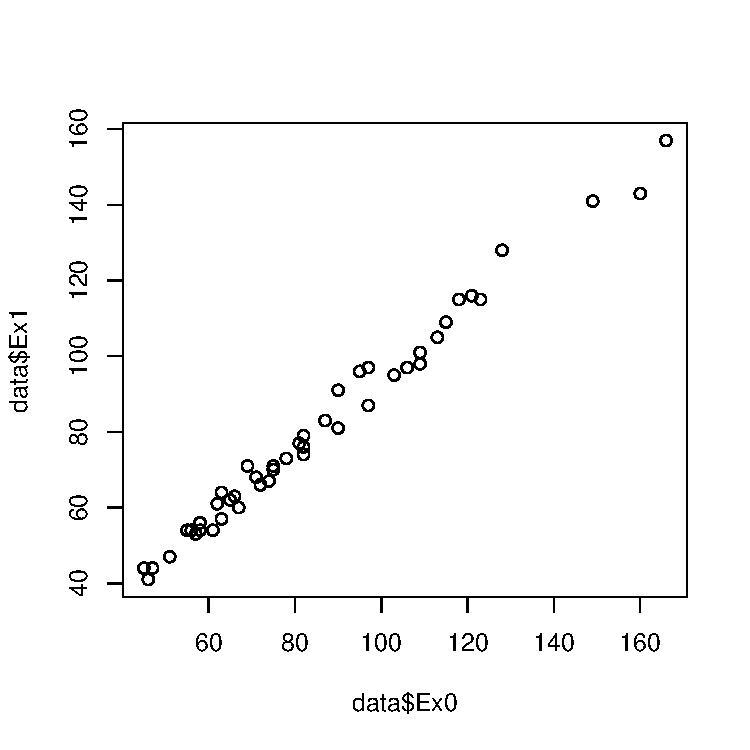
\includegraphics[width=.9\textwidth]{part10-pairs.pdf}

\begin{verbatim}
> # SS involving 'Ex0' and 'Ex1'.
> sse.full <- deviance(myfit)
> 
> myfit.red <- update(myfit, . ~ . - Ex0 - Ex1)
>     # Drop 'Ex0' and 'Ex1'.
> sse.red <- deviance(myfit.red)
> 
> myfit.ex0 <- update(myfit.red, . ~ . + Ex0)
>     # Include 'Ex0', but not 'Ex1'.
> myfit.ex1 <- update(myfit.red, . ~ . + Ex1)
>     # Include 'Ex1', but not 'Ex0'.
> 
> sse.ex0 <- deviance(myfit.ex0)
> sse.ex1 <- deviance(myfit.ex1)
\end{verbatim}

Now let's observe some typical patterns in SS
in the situation of multicollinearity.
(Also note how we calculate various SSR.)

\begin{verbatim}
> # SSR(Ex0 | others but not Ex1)
> print(sse.red - sse.ex0)
[1] 8106.567
> 
> # SSR(Ex0 | others incl. Ex1)
> # This should be much smaller than the above,
> # if 'Ex1' is highly correlated with 'Ex0'.
> print(sse.ex1 - sse.full)
[1] 1109.830
> 
> # SSR(Ex1 | others but not Ex0)
> print(sse.red - sse.ex1)
[1] 7159.075
> 
> # SSR(Ex1 | others incl. Ex0)
> # This should be much smaller than the above,
> # if 'Ex1' is highly correlated with 'Ex0'.
> print(sse.ex0 - sse.full)
[1] 162.338
> 
> # SSR(Ex0, Ex1 | others)
> # This should be much smaller than
> #   SSR(Ex0 | others but not Ex1)
> #   +
> #   SSR(Ex1 | others but not Ex0)
> # if 'Ex0' and 'Ex1' are highly correlated,
> # because these two SSR have much in common.
> print(sse.red - sse.full)
[1] 8268.905
>     # Indeed, this is just slightly larger than either
>     # of those two SSR's.
\end{verbatim}

Which predictors would be significant
if we performed a `t' test?
This can be seen from the $P$ value column of the
\verb+coefficients+ block of the output of \verb+summary+:
\begin{verbatim}
> print(summary(myfit)$coefficients, digits = 2)
            Estimate Std. Error t value Pr(>|t|)
(Intercept) -6.9e+02    155.888   -4.44  9.6e-05
Age          1.0e+00      0.423    2.46  1.9e-02
S           -8.3e+00     14.912   -0.56  5.8e-01
Ed           1.8e+00      0.650    2.77  9.1e-03
Ex0          1.6e+00      1.059    1.52  1.4e-01
Ex1         -6.7e-01      1.149   -0.58  5.7e-01
LF          -4.1e-02      0.153   -0.27  7.9e-01
M            1.6e-01      0.210    0.78  4.4e-01
N           -4.1e-02      0.130   -0.32  7.5e-01
NW           7.2e-03      0.064    0.11  9.1e-01
U1          -6.0e-01      0.437   -1.38  1.8e-01
U2           1.8e+00      0.856    2.09  4.4e-02
W            1.4e-01      0.106    1.30  2.0e-01
X            7.9e-01      0.235    3.37  1.9e-03
\end{verbatim}
Turns out quite a few predictors are insignificant
($P \text{ value } > 0.05$).
But if we just focus on \verb+Ex0+ and \verb+Ex1+,
they are also insignificant.
We could have done a $F$ test for these two predictors
and see whether they as a group are significant.

Now let's calculate the VIF of \verb+Ex0+ and \verb+Ex1+
(actually we'll get the VIF of all the predictors).
To this end we need the correlation matrix of the predictors.
This is calculated by the \texttt{R} function
\verb+cor+, which takes a matrix and treats each column as a variable
and each row as a case (or observation), and outputs pairwise
correlations in a matrix.
We will need the diagonal elements of the inverse of this correlation
matrix. The diagonal elements of a square matrix is extracted by
\verb+diag+.

\begin{verbatim}
> # VIF
> # Get the design matrix.
> # This is the data.frame with all X columns,
> # including the intercept column, i.e. the column
> # of 1's (which is the first column).
> X <- model.matrix(myfit)
> 
> cc <- cor(X[, -1])
>     # Correlation matrix, excluding the intercept column.
> print(diag(solve(cc)))
      Age         S        Ed       Ex0       Ex1        LF         M         N 
 2.698021  4.876751  5.049442 94.633118 98.637233  3.677557  3.658444  2.324326 
       NW        U1        U2         W         X 
 4.123274  5.938264  4.997617  9.968958  8.409449 
>     # 'solve' finds the inverse.
>     # 'diag' extracts diagonal elements.
\end{verbatim}

Note that our suspects have especially large VIF's.

\end{document}

